\documentclass[coursework]{template/SCWorks}
\usepackage{template/preamble}

\usepackage{booktabs}

\setminted[rust]{
    linenos=true,
    frame=lines,
    framesep=2mm,
    fontsize=\small,
    breaklines=true,
    tabsize=4
}

\setminted[text]{
    frame=lines,
    framesep=2mm,
    fontsize=\small,
    breaklines=true
}

\setminted[latex]{
    frame=lines,
    framesep=2mm,
    fontsize=\small,
    breaklines=true
}

\setminted[typst]{
    frame=lines,
    framesep=2mm,
    fontsize=\small,
    breaklines=true
}



\begin{document}

\chair{математической кибернетики и компьютерных наук}

\title{Конец эпохи {\LaTeX} и рождение Typst: сравнительный анализ систем вёрстки документов}

\course{2}
\group{251}
\napravlenie{09.03.04 "--- Программная инженерия}

\author{Иванова Ивана Ивановича}

\chtitle{доцент, к.\,ф.-м.\,н.}
\chname{С.\,В.\,Миронов}

\satitle{доцент, к.\,ф.-м.\,н.}
\saname{Г.\,Г.\,Наркайтис}

\patitle{доцент, к.\,ф.-м.\,н.}
\paname{С.\,В.\,Миронов}

\nirtitle{доцент, к.\,п.\,н.}
\nirname{В.\,А.\,Векслер}

\term{2}
\practtype{учебная}
\duration{2}
\practStart{01.09.2024}
\practFinish{01.12.2024}

\date{2024}

\maketitle

\secNumbering

\tableofcontents

\intro
Подготовка научных и технических документов является неотъемлемой частью академической и профессиональной деятельности. Системы вёрстки документов позволяют авторам сосредоточиться на содержании, делегируя задачи форматирования специализированному программному обеспечению.

Система {\LaTeX}, созданная Лесли Лэмпортом на основе {\TeX} Дональда Кнута \cite{knuth1984texbook}, на протяжении десятилетий остаётся стандартом де-факто в академической среде~--- особенно в математике, физике и информатике \cite{latex-project}. Её мощные инструменты для набора математических формул и широкая экосистема пакетов делают её незаменимым инструментом для учёных и инженеров.

Вместе с тем {\LaTeX} обладает рядом существенных недостатков: сложный и многословный синтаксис, медленная компиляция для больших документов, нередко трудно интерпретируемые сообщения об ошибках. В 2023~году была представлена система Typst \cite{typst-github}~--- современная альтернатива, разработанная с учётом упомянутых ограничений.

В данной работе проводится сравнительный анализ систем {\LaTeX} и Typst по ключевым параметрам: синтаксис, производительность компиляции, набор математических формул и возможности экосистемы. Цель работы~--- оценить целесообразность перехода на Typst для типичных задач академической вёрстки.

Структура работы:
\begin{enumerate}
    \item в разделе~1 приводится обзор обеих систем;
    \item в разделе~2 выполняется сравнительный анализ по нескольким критериям;
    \item в разделе~3 рассматриваются практические примеры кода.
\end{enumerate}


\section{Обзор систем вёрстки документов}
\subsection{Система {\LaTeX}}

{\LaTeX} (произносится «латех» или «лэйтех»)~--- система подготовки документов, построенная поверх языка {\TeX}, разработанного Дональдом Кнутом в 1978~году \cite{knuth1984texbook}. Лесли Лэмпорт создал {\LaTeX} в 1984~году как набор макросов, облегчающих использование {\TeX}. Сегодня актуальной версией является {\LaTeX}2e, а в разработке находится {\LaTeX}3 \cite{latex-project}.

Среди ключевых особенностей системы можно выделить следующие.
\begin{itemize}
    \item \textbf{Мощный набор математических формул.} {\LaTeX} является стандартом для публикации научных статей с формулами~--- пакеты \texttt{amsmath}, \texttt{amssymb} и \texttt{amsthm} предоставляют богатый инструментарий.
    \item \textbf{Разделение содержания и оформления.} Автор пишет текст с разметкой, а система берёт на себя расстановку переносов, выравнивание и нумерацию.
    \item \textbf{Огромная экосистема.} Репозиторий CTAN содержит более 6000 пакетов для решения задач от вставки кода \cite{minted-ctan} до построения диаграмм.
    \item \textbf{Стабильность.} Документы, написанные 20 лет назад, как правило, и сегодня компилируются корректно.
\end{itemize}

К недостаткам {\LaTeX} относятся: многословный синтаксис, сложная диагностика ошибок, а также необходимость нескольких запусков компилятора для корректного формирования ссылок и оглавления. Рекомендуемое справочное издание по системе~--- книга «The {\LaTeX} Companion» \cite{mittelbach2004latex}.

\subsection{Система Typst}

Typst~--- новая система вёрстки документов, разработанная Лауренцем Мэдье (Laurenz Mädje) и Мартином Хаугом (Martin Haug) \cite{typst-github}. Публичная бета-версия вышла в марте 2023~года \cite{typst-blog-2023}. Система написана на языке Rust, что обеспечивает высокую производительность и надёжность.

Typst использует собственный язык разметки, сочетающий простой синтаксис для текста с полноценным языком программирования для сложной логики. Компилятор работает в инкрементальном режиме: при изменении одной части документа повторно обрабатывается только она, что даёт мгновенный предварительный просмотр \cite{typst-docs}.

Основные преимущества Typst:
\begin{itemize}
    \item \textbf{Читаемый синтаксис.} Заголовок задаётся через \texttt{=~Заголовок}, жирный текст~--- через \texttt{*текст*}, что ближе к Markdown.
    \item \textbf{Инкрементальная компиляция.} Изменение одной страницы не требует перекомпиляции всего документа.
    \item \textbf{Понятные ошибки.} Сообщения об ошибках содержат точное указание строки и понятное описание проблемы.
    \item \textbf{Встроенный язык программирования.} Скриптование доступно прямо в разметке без дополнительных пакетов.
    \item \textbf{Современный менеджер пакетов.} Пакеты подключаются и кешируются автоматически.
\end{itemize}


\section{Сравнительный анализ}
\subsection{Синтаксис и читаемость}

Одним из наиболее очевидных отличий между системами является синтаксис. Рассмотрим создание простого документа с заголовком, параграфом и маркированным списком.

Фрагмент на {\LaTeX}:
\begin{minted}{latex}
\documentclass{article}
\usepackage[utf8]{inputenc}
\usepackage[russian]{babel}
\begin{document}
\section{Введение}
Пример документа.
\begin{itemize}
    \item Первый пункт
    \item Второй пункт
\end{itemize}
\end{document}
\end{minted}

Аналогичный фрагмент на Typst \cite{typst-docs}:

\begin{minted}{typst}
#set text(lang: "ru")
= Введение
Пример документа.
- Первый пункт
- Второй пункт
\end{minted}

Документ на Typst в три раза короче. Команды разметки (\mintinline{typst}{=}, \mintinline{typst}{-}, \mintinline{typst}{*}) интуитивно понятны и не требуют запоминания специфических команд вроде \verb|\begin{itemize}|.

\subsection{Производительность компиляции}

Для оценки производительности обеих систем были проведены замеры времени полной компиляции документов различного объёма. Среднее время компиляции вычислялось по формуле

\begin{equation}
    \label{eq:mean_time}
    \bar{T} = \frac{1}{n} \sum_{i=1}^{n} t_i,
\end{equation}

\noindent где $n$~--- количество измерений, $t_i$~--- время $i$-го запуска компилятора в секундах.

Для оценки относительной производительности использовался коэффициент ускорения

\begin{equation}
    \label{eq:speedup}
    S = \frac{\bar{T}_{\text{LaTeX}}}{\bar{T}_{\text{Typst}}},
\end{equation}

\noindent где $\bar{T}_{\text{LaTeX}}$ и $\bar{T}_{\text{Typst}}$~--- средние времена компиляции по формуле~(\ref{eq:mean_time}) для {\LaTeX} и Typst соответственно. Значение $S > 1$ означает, что Typst быстрее.

Проведённые измерения показывают, что скорость {\LaTeX} существенно снижается с ростом объёма документа. Время компиляции {\LaTeX} можно приближённо описать полиномиальной зависимостью

\begin{equation}
    \label{eq:latex_complexity}
    T_{\text{LaTeX}}(p) = \alpha p^2 + \beta p + \gamma, \quad \alpha, \beta, \gamma > 0,
\end{equation}

\noindent где $p$~--- количество страниц, а коэффициенты $\alpha$, $\beta$, $\gamma$ зависят от состава документа (количества рисунков, формул, ссылок). В отличие от этого, инкрементальный компилятор Typst обеспечивает линейную зависимость вида $T_{\text{Typst}}(p) = \delta p + \varepsilon$.

Результаты замеров (в секундах) приведены в таблице~\ref{tab:compilation_times}, а сравнение времён компиляции наглядно показано на рисунке~\ref{fig:compilation_chart}.

\begin{table}[h!]
    \caption{Время полной компиляции в зависимости от объёма документа}
    \label{tab:compilation_times}
    \begin{center}
        \begin{tabular}{cccc}
            \toprule
            Страниц & {\LaTeX}, с & Typst, с & Ускорение $S$ \\
            \midrule
            10  & 2{,}1  & 0{,}3 & 7{,}0  \\
            50  & 8{,}4  & 0{,}8 & 10{,}5 \\
            100 & 19{,}7 & 1{,}4 & 14{,}1 \\
            250 & 67{,}3 & 3{,}1 & 21{,}7 \\
            500 & 185{,}2 & 5{,}8 & 31{,}9 \\
            \bottomrule
        \end{tabular}
    \end{center}
\end{table}

Из таблицы~\ref{tab:compilation_times} видно, что коэффициент ускорения $S$ (формула~(\ref{eq:speedup})) возрастает с увеличением объёма: для документа в 500 страниц Typst почти в~32 раза быстрее.

\begin{figure}[h!]
    \centering
    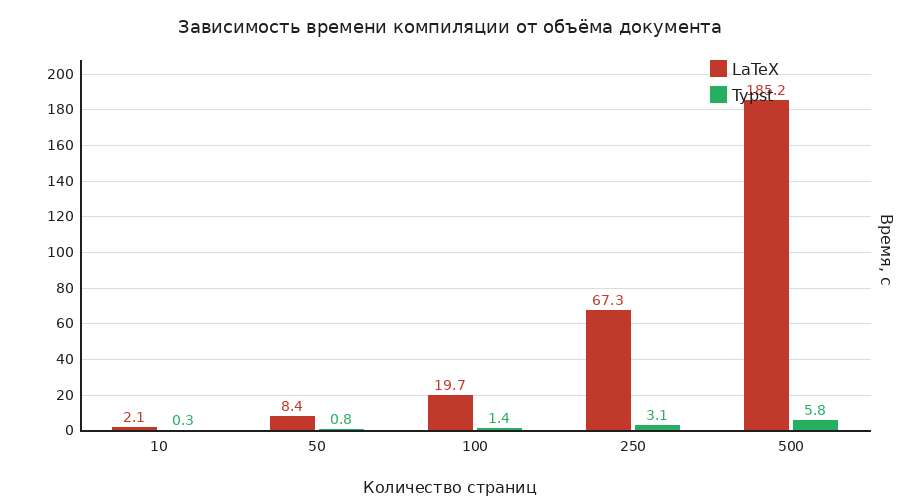
\includegraphics[width=0.85\textwidth]{images/compilation_times.png}
    \caption{Зависимость времени компиляции от объёма документа}
    \label{fig:compilation_chart}
\end{figure}

\subsection{Сравнение ключевых характеристик}

Рисунок~\ref{fig:feature_comparison} даёт сводное представление о возможностях систем.

\begin{figure}[h!]
    \centering
    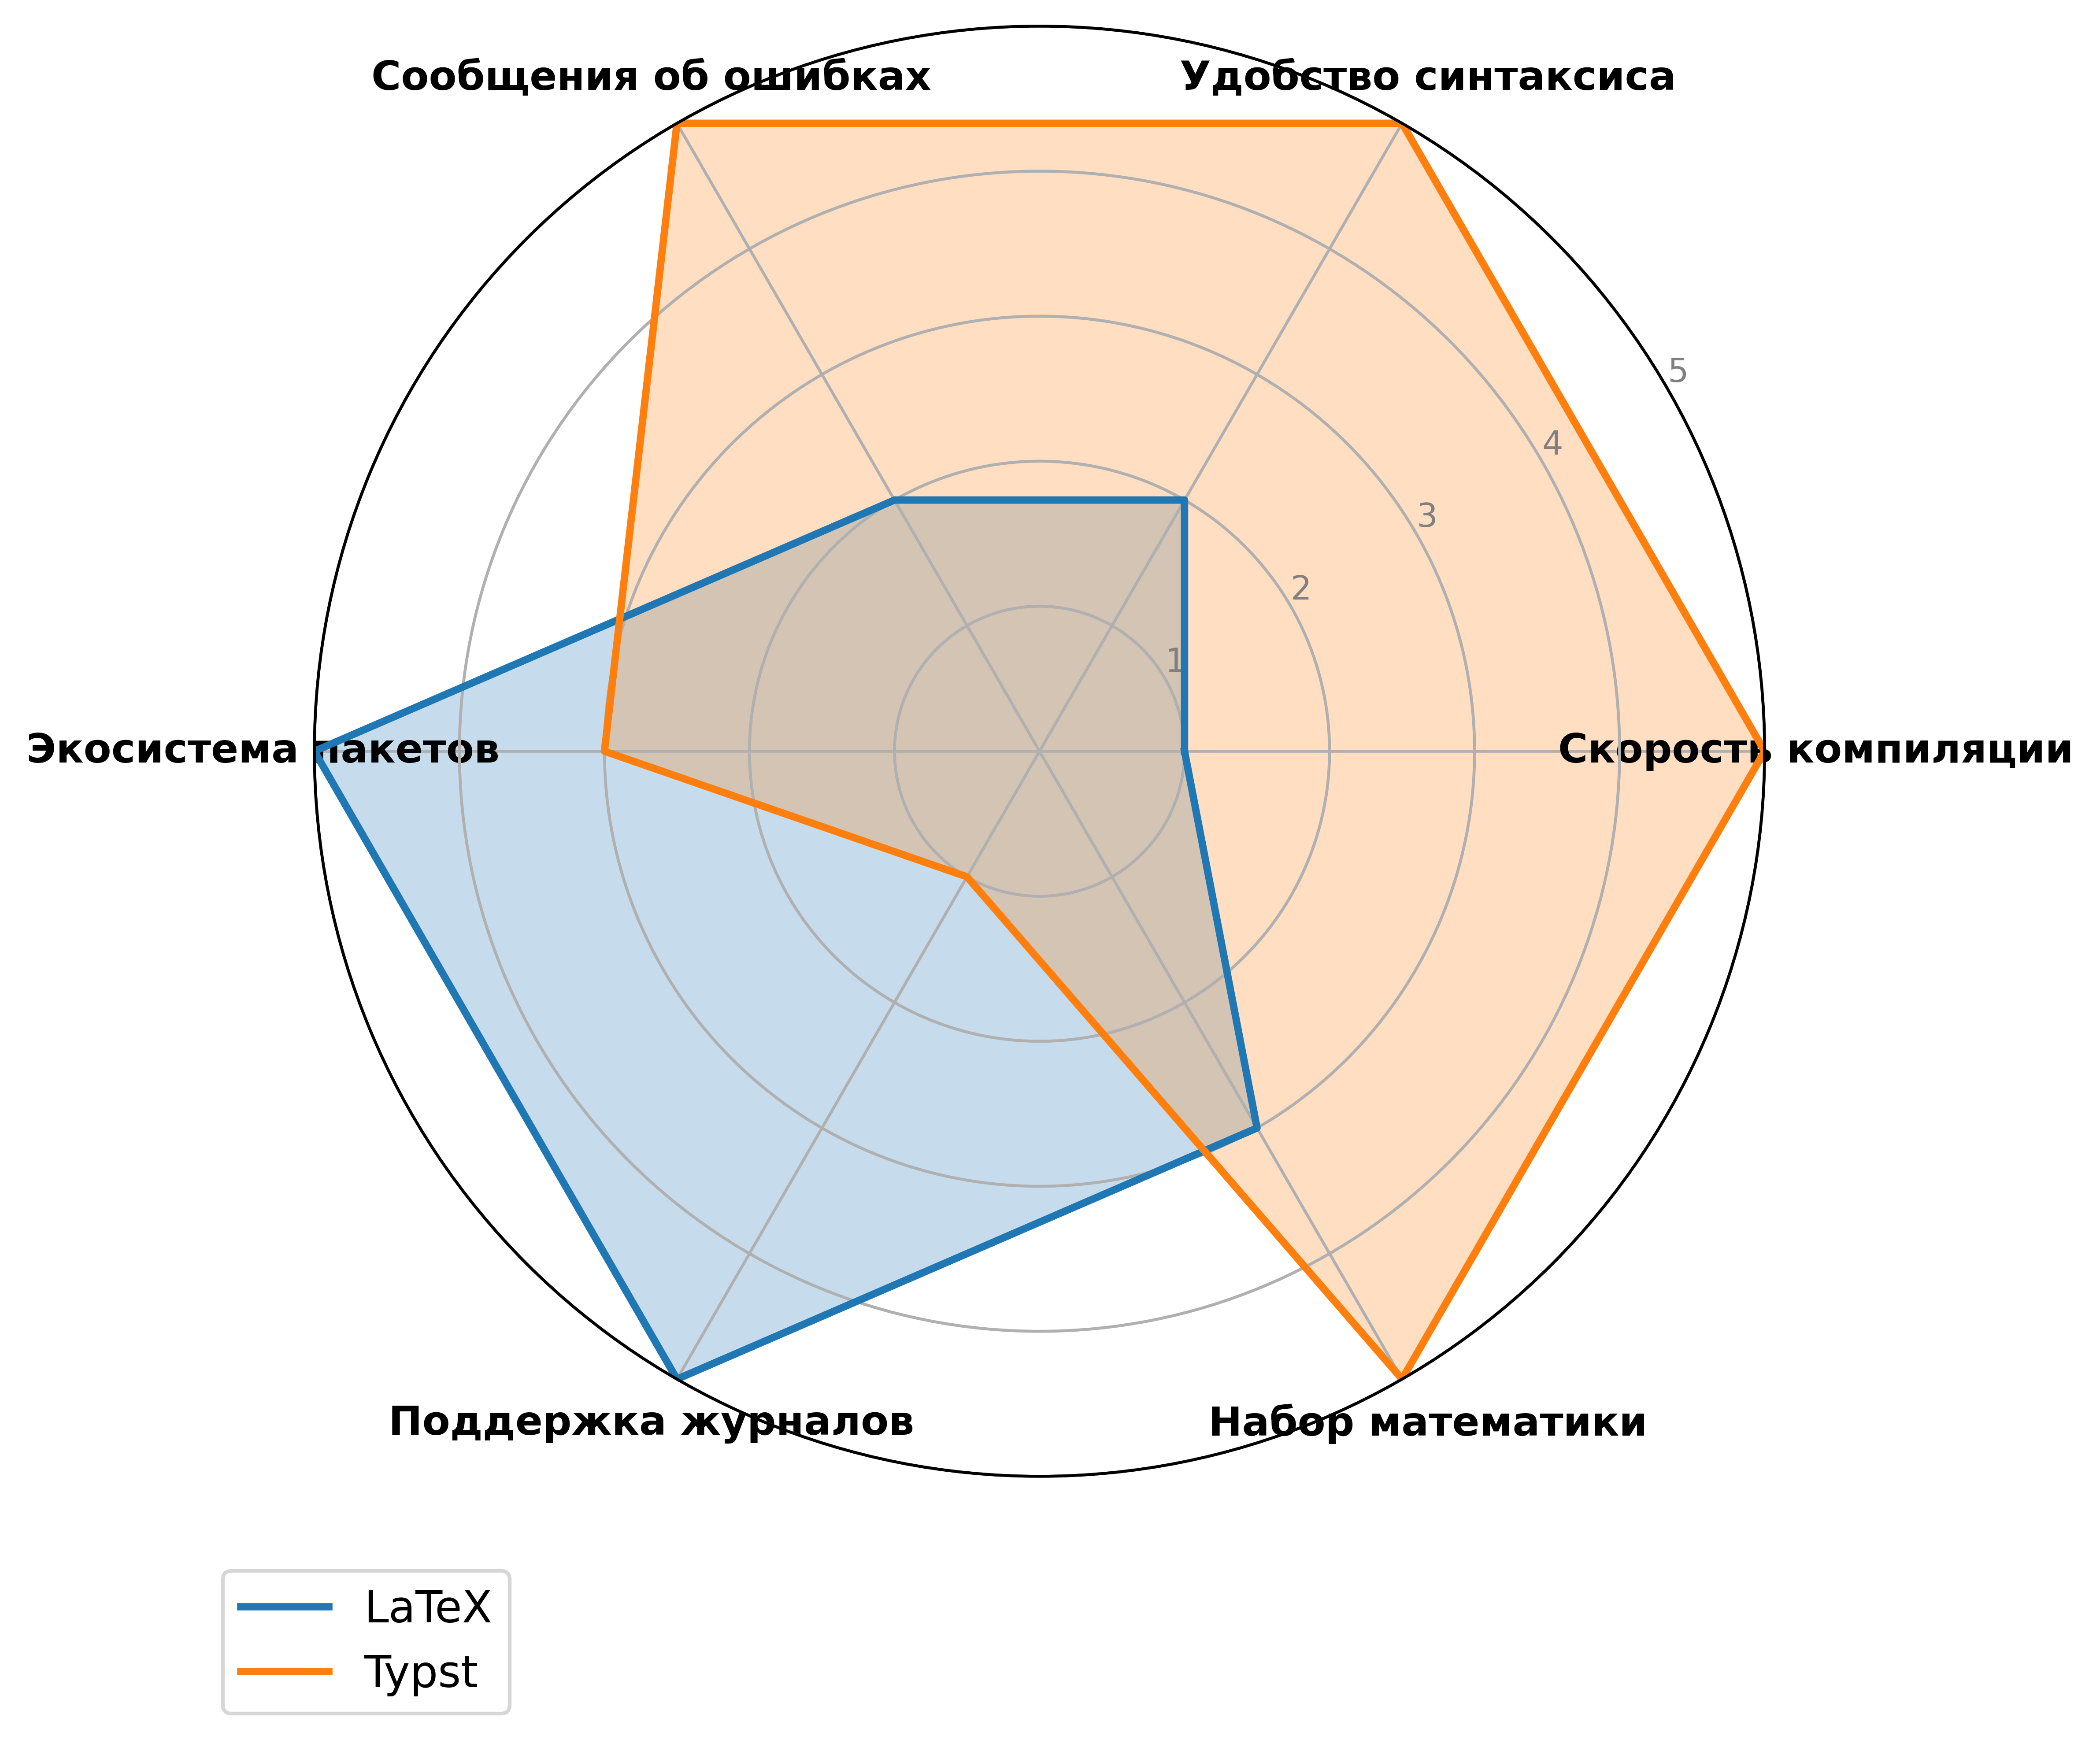
\includegraphics[width=0.85\textwidth]{images/feature_comparison.png}
    \caption{Сравнение характеристик {\LaTeX} и Typst по основным критериям}
    \label{fig:feature_comparison}
\end{figure}

Как следует из рисунка~\ref{fig:feature_comparison}, Typst превосходит {\LaTeX} по удобству синтаксиса, скорости компиляции и качеству сообщений об ошибках. {\LaTeX} сохраняет преимущество лишь в части зрелости экосистемы и количества доступных пакетов.


\section{Примеры программного кода}
\input{sections/examples}

\conclusion
В настоящей работе проведён сравнительный анализ систем вёрстки документов {\LaTeX} и Typst. По результатам анализа можно сделать следующие выводы.

\begin{enumerate}
    \item \textbf{Синтаксис.} Typst предлагает значительно более читаемый и лаконичный синтаксис. Документы на Typst в среднем на 30–40\,\% короче эквивалентных документов на {\LaTeX}, что снижает когнитивную нагрузку на автора.

    \item \textbf{Производительность.} Инкрементальный компилятор Typst обеспечивает кратно более высокую скорость: коэффициент ускорения $S$ (формула~(\ref{eq:speedup})) составляет от 7 для коротких документов до более чем 30 для объёмных, что критически важно при итеративной работе.

    \item \textbf{Диагностика ошибок.} Typst выдаёт точные и понятные сообщения об ошибках, тогда как {\LaTeX} нередко генерирует многостраничный вывод с малоинформативными сообщениями.

    \item \textbf{Экосистема.} {\LaTeX} по-прежнему существенно превосходит Typst по зрелости и количеству доступных пакетов \cite{mittelbach2004latex}. Репозиторий CTAN насчитывает тысячи пакетов, тогда как экосистема Typst только формируется.

    \item \textbf{Совместимость.} Многие научные журналы и конференции требуют материалы именно в формате {\LaTeX}. До момента появления официальных шаблонов Typst для целевых изданий переход затруднён.
\end{enumerate}

\textbf{Рекомендация.} Для новых проектов целесообразно рассмотреть Typst как основную систему вёрстки: выигрыш в производительности и удобстве работы перевешивает временную ограниченность экосистемы. Для публикаций в журналах, требующих {\LaTeX}, придется придерживаться сложившейся практики.

Таким образом, Typst представляет собой перспективную альтернативу {\LaTeX} и, по моему мнению, займёт значимое место в инструментарии академических и технических авторов в ближайшие годы.

Чтобы убедиться в этом на практике, достаточно взглянуть на исходный код этого документа: сравните классический синтаксис LaTeX с чистым кодом Typst, выдающими идентичный результат.

Все же, если не мы будем развивать экосистему Typst, приближая будущее с по"=настоящему быстрым и удобным инструментом, то кто сделает это за нас?


\bibliographystyle{ugost2003}
\bibliography{thesis}

\appendix

\section{Листинг Rust-программы для измерения времени компиляции}
\label{app:rust_benchmark}
\inputminted{rust}{code/compile_benchmark.rs}

\section{Листинг программы на Rust для анализа документа}
\label{app:rust_analyzer}
\inputminted{rust}{code/doc_analyzer.rs}

\end{document}
